\documentclass[14pt,a4paper]{article}
\usepackage{ucs}
\usepackage{fancyhdr}
\usepackage{listings}
\usepackage{amsfonts}
\usepackage{amsmath}
\usepackage{setspace}
\usepackage{graphicx}
\usepackage{amssymb}
\usepackage{array}
\usepackage{subfigure}
\usepackage{listing}

\pagestyle{fancy}
\renewcommand\thesubsubsection{}
\renewcommand\thesubsection{\alph{subsection})}
\renewcommand\thesection{Exercise \arabic{section}}
\lhead{Exercise 3}
\rhead{Group 4}
\title{\textbf{Sheet 3} \\  \textbf{Robot Control}}
\author{Group 4 \\Urs Borrmann, Caner Hazirbas, FangYi Zhi}

\begin{document}
\maketitle
\onehalfspacing

\section{}
	\subsection{Specify the control law of a PID controller}
	$$
		u(t)=K_P \  e(t) + K_D \ \dot{e}(t) + K_I \int_{-\infty}^t e(t)\,dt.
	$$
	
	\subsection{Define how the error integral can be computed in the discrete case}
	\begin{eqnarray*}
		e_{I,t}&=&e_{I,t-1}+e_{t}. \\
		e_{I,0}&=&0.
	\end{eqnarray*}
	
	\subsection{Define a formula for the discrete error derivative}
	$$
		e_{D,t}=e_t - e_{t-1}
	$$
	
	\subsection{Specify the discrete PID control law}
	$$
		u_t=K_P \ e_t + K_D \ e_{D,t}+K_I \ e_{I,t}
	$$
	
	\refstepcounter{subsection}
	\subsection{Specify how the error signals for each of these controllers can be computed from the current pose and the goal pose}
				\[\vec{e}= \left( \begin{array}{c}
						x_{e} \\ y_{e}\\ \psi_e 
				\end{array}\right) , \vec{x}= \left( \begin{array}{c}
						x_{x} \\ y_{x}\\ \psi_x 
				\end{array}\right), \vec{g}= \left( \begin{array}{c}
						x_{g} \\ y_{g}\\ \psi_g 
				\end{array}\right)\] 	
		$$
				\vec{e} = \vec{g} - \vec{x}
		$$
				\[\left( \begin{array}{c}
						x_{e} \\ y_{e}\\ \psi_e 
				\end{array}\right)= \left( \begin{array}{c}
						x_{g} - x_{x} \\ y_{g}- y_{x} \\ \psi_g - \psi_x 
				\end{array}\right)\] 
				
	\refstepcounter{subsection}
	\subsection{Screenshol of RVIZ}
	\begin{figure}[htbp]
	\centering
	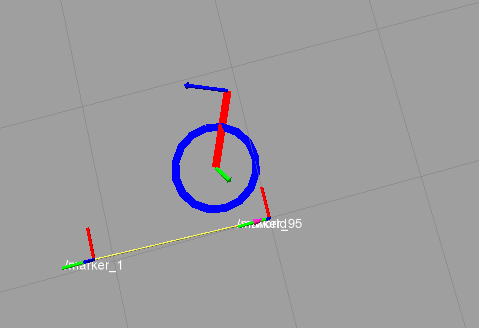
\includegraphics[scale=0.7]{control_flight.png}
  	\caption{screenshot from RVIZ to indicate the x,y,yaw control command}
    \label{graph:RVIZ control}
	\end{figure}
	
\end{document}
